
\documentclass[8pt]{beamer}

\usepackage[english]{babel}
\usepackage[utf8]{inputenc}
\usepackage{pdfpages}
\usepackage{color}
\usepackage{graphicx, import}
\usepackage{amsmath}
\usepackage{amssymb}
\usepackage{physics} % norm
\usepackage{tikz}
\usepackage{tkz-euclide}
\usepackage{enumitem}
\usepackage{pgfplots}
\usepackage{multicol}
\usepackage{tabularx}
\usepackage[numbers, square]{natbib}
\usepackage{mathtools}
\usepackage{transparent}
\usepackage{caption} % change style of figure 
\usepackage{subcaption}
\usepackage{booktabs}
\usepackage[super]{nth}

\captionsetup*[subfigure]{position=bottom}


\usetikzlibrary{positioning, fit, patterns, snakes, chains, arrows, decorations.markings, arrows.meta}
%\tikzexternalize[prefix=out/figures/]
\newcolumntype{Y}{>{\centering\arraybackslash}X} % centered equidistant columns

\bibliographystyle{plainnat}
\usetheme{metropolis}
\setbeamertemplate{frame footer}{\insertshortauthor\hfill\insertshortinstitute}
\setbeamercolor{footline}{fg=gray}

\newcommand{\cX}{\mathcal{X}}
\newcommand{\cY}{\mathcal{Y}}
\newcommand{\cL}{\mathcal{L}}
\newcommand{\cH}{\mathcal{H}}
\newcommand{\cV}{\mathcal{V}}
\newcommand{\cA}{\mathcal{A}}
\newcommand{\cF}{\mathcal{F}}
\newcommand{\R}{\mathbb{R}}
\newcommand{\I}{\mathrm{I}}
\newcommand{\cl}{\mathcal{l}}

\newcommand{\fL}{\mathfrak{L}}
\newcommand{\fH}{\mathfrak{H}}
\newcommand{\fV}{\mathfrak{V}}

\renewcommand{\epsilon}{\varepsilon}

\newcommand{\dK}{\mathbb{K}}

\newcommand{\closure}{\mathrm{\mathbf{cl}}}

\newcommand{\bGamma}{\mathbf{\Gamma}}

\DeclareMathOperator*{\argmax}{arg\,max}
\DeclareMathOperator*{\argmin}{arg\,min}
\newcommand{\T}{\mathrm{T}}


\title[]{Mechanical Regression for Supervised Learning}
\author[Nikolas Klug]{Nikolas Klug}
\institute[University of Augsburg]{University of Augsburg}
\date{\nth{25} March 2021}


\begin{document}
	{
	\setbeamertemplate{footline}{}
	\begin{frame}
		\titlepage
	\end{frame}
	}
	\addtocounter{framenumber}{-1}

	\begin{frame}{Source}
		\textbf{Do Ideas Have Shape? Plato's Theory of Forms as the Continuous Limit of Artificial Neural Networks}\linebreak
		\begin{footnotesize}
			Houman Owhadi.\linebreak
			arXiv preprint arXiv:2008.03920, August 2020.
		\end{footnotesize}
	\end{frame}

	\begin{frame}{Supervised Learning}
		\textbf{Supervised Learning Problem}:\\
		Given data pairs $(X_i, Y_i)$ and $f^\dagger(X_i) = Y_i$ for $1 \leq i \leq N$,
		approximate $f^\dagger$.
		\\~\\
		In our setting:\\
		$X_i \in \cX$, $Y_i \in \cY$, where $\cX$ and $\cY$ are Hilbert Spaces.\\
		Shorthand notation: $f^\dagger(X) = Y$.
	\end{frame}

	\begin{frame}{Residual Neural Networks}
		Instead of the direct mapping $f: \cX \rightarrow \cX$, learn the residual mapping 
		\begin{gather*}
			g: \cX \rightarrow \cX\\
			g(x) \coloneqq f(x) - x \ .
		\end{gather*}
		\begin{figure}
	\centering
	\scalebox{0.9}{
	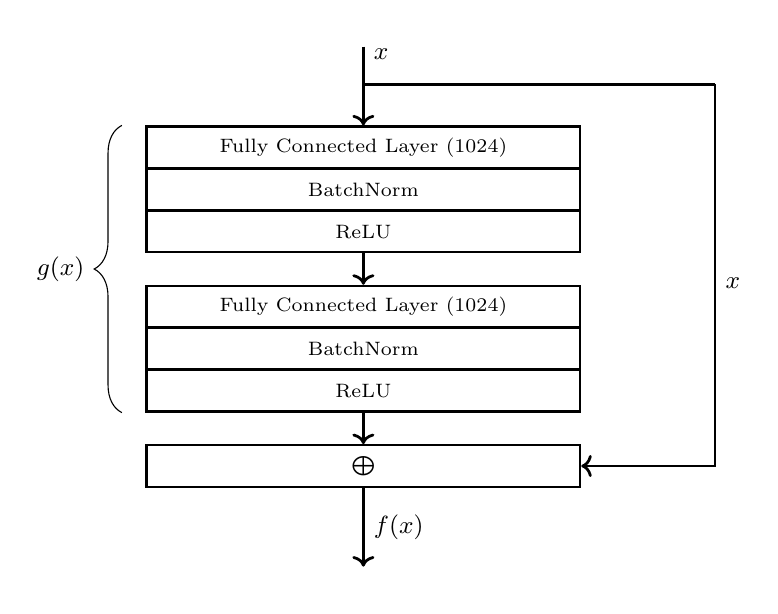
\begin{tikzpicture}
		[
		font=\scriptsize,
		block/.style ={rectangle, draw=black, thick, text width=15em, align=center, minimum height=1.5em}
		]
		\node[] (a) [block] {Fully Connected Layer (1024)};
		\node[below= -1.5\pgflinewidth of a] (a1) [block] {BatchNorm};
		\node[below= -1.5\pgflinewidth of a1] (b) [block] {ReLU};
		\node[below= 4mm of b] (c) [block] {Fully Connected Layer (1024)};
		\node[below= -1.5\pgflinewidth of c] (c1) [block] {BatchNorm};
		\node[below= -1.5\pgflinewidth of c1] (d) [block] {ReLU};
		\node[below= 4mm of d] (e) [block] {$\bigoplus$};
		\node[above=of a] (x) [] {};
		\draw[->, line width=1pt] (b.south) -- (c.north);
		\draw[->, line width=1pt] (d.south) -- (e.north);
		\draw[->, line width=1pt] (x) -- node [pos=0.1, right] {\small $x$} (a);
		\node[below=of e] (y) [] {};
		\draw[->, line width=1pt] (e) -- node [midway, right] {\small $f(x)$} (y);
		\node[above=.4 of a] (z) [] {};
		\node[right=12em of z] (h) [] {};
		\draw[line width=1pt] (z.center) -- (h.center);
		\draw[->, line width=1pt] (h.center) |- node [pos=.26,right] {\small $x$} (e.east);
		\draw [decorate, decoration={brace, amplitude=10pt}] ([xshift=-0.3cm]d.south west)-- ([xshift=-0.3cm]a.north west) node [black,midway, left, xshift=-10pt]{\small $g(x)$};
	\end{tikzpicture}
}
	\label{fig:residual-block}
\end{figure}
	\end{frame}

	\begin{frame}[t]{Simplified Model of ResNets}
		$\cV$: Reproducing Kernel Hilbert Space (RKHS) of functions $v: \cX \rightarrow \cX$\\
		$\cH$: RKHS of functions $f: \cX \rightarrow \cY$\\
		$l: \cY \times \cY \rightarrow [0, \infty)$: loss function\\
		$\nu, \lambda > 0$: balancing parameters\\
		\vspace{1cm}
		\textbf{Discrete ResNet:}
		\begin{equation*}
			\label{prob:min-v-f}
			\begin{cases}
				\text{Minimize~} & \nu \cdot \frac{L}{2} \sum_{k=1}^{L} \norm{v_k}_\cV^2
				+ \lambda \norm{f}_\cH^2 
				+ l((f \circ \Phi_L)(X), Y) \\
				\text{such that~} & v_1, \ldots, v_L \in \cV, f \in \cH \ .
			\end{cases}
		\end{equation*}
		
		\uncover<2->{
		Or alternatively:
		\begin{equation*}
			\label{prob:discrete-resnet}
			\begin{cases}
				\text{Minimize~} & \nu \cdot \frac{L}{2} \sum_{k=1}^{L} \norm{v_k}_\cV^2
				+ l_R(\Phi_L(X), Y) \\
				\text{such that~} & v_1, \ldots, v_L \in \cV\ .
			\end{cases}
		\end{equation*}
		where $l_R(X, Y) \coloneqq \inf_{f \in \mathcal{H}} \lambda \norm{f}_\mathcal{H}^2 + l (f(X), Y)$.
	}
	\end{frame}

	\begin{frame}[t]{Discrete Least Action}
		\textbf{Discrete ResNet:}
		\begin{equation*}
			\label{prob:discrete-resnet}
			\begin{cases}
				\text{Minimize~} & \nu \cdot \frac{L}{2} \sum_{k=1}^{L} \norm{v_k}_\cV^2
				+ l_R(\Phi_L(X), Y) \\
				\text{such that~} & v_1, \ldots, v_L \in \cV\ .
			\end{cases}
		\end{equation*}
		Define 
		\begin{align*}
			q_1 &\coloneqq X\\
			q_k &\coloneqq ((I + v_{k-1}) \circ \ldots \circ (I + v_1)) (X) \ .
		\end{align*}
		\uncover<2->{
			Then
			\begin{equation}
				q_{k+1} = v_k(q_k) + q_k
			\end{equation}
			and $\norm{v_k}_\cV^2$ can be represented as
			\begin{equation}
				\norm{v_k}_\cV^2 = (q_{k+1} - q_k)^\mathrm{T} \bGamma(q_k, q_k)^{-1} (q_{k+1} - q_k) \ ,
			\end{equation}
			where $\bGamma: \cX \times \cX \rightarrow L(\cX, \cX)$ is the reproducing kernel associated with the RKHS $\cV$.\\
		}
		\uncover<3->{
			\textbf{Discrete Least Action:}
			\begin{equation*}
			\label{prob:min-q}
				\begin{cases}
					\text{Minimize~} & \nu \cdot \frac{1}{2} \sum_{k=1}^{L} \left(\frac{q_{k+1} - q_k}{\Delta t}\right)^\mathrm{T} \bGamma(q_k, q_k)^{-1} \left(\frac{q_{k+1} - q_k}{\Delta t}\right) \Delta t+ l(q_{L+1}, Y) \\
					\text{such that~} & q_1 = X,\ q_2, \ldots, q_{L+1} \in \cX^N  \text{~and~} \Delta t = \frac{1}{L} \ .
				\end{cases}
		\end{equation*}
		}
	\end{frame}
	
	\begin{frame}{Continuous Least Action}
				\textbf{Discrete Least Action:}
		\begin{equation*}
		\label{prob:min-q}
		\begin{cases}
		\text{Minimize~} & \nu \cdot \frac{1}{2} \sum_{k=1}^{L} \left(\frac{q_{k+1} - q_k}{\Delta t}\right)^\mathrm{T} \bGamma(q_k, q_k)^{-1} \left(\frac{q_{k+1} - q_k}{\Delta t}\right) \Delta t+ l(q_{L+1}, Y) \\
		\text{such that~} & q_1 = X,\ q_2, \ldots, q_{L+1} \in \cX^N  \text{~and~} \Delta t = \frac{1}{L} \ .
		\end{cases}
		\end{equation*}
		
		Idea:
		\begin{equation*}
			\left(\frac{q_{k+1} - q_k}{\Delta t}\right)^\mathrm{T} \bGamma(q_k, q_k)^{-1} \left(\frac{q_{k+1} - q_k}{\Delta t}\right) 
			\approx \dot{q}(t)^\T \bGamma(q(t), q(t))^{-1} \dot{q}(t)
		\end{equation*}
		Define
		\begin{equation*}
			\fL(t, q(t), \dot{q}(t)) \coloneqq \frac{1}{2} \dot{q}(t)^\T \bGamma(q(t), q(t))^{-1} \dot{q}(t) \ .
		\end{equation*}
		\uncover<2->{
		\textbf{Continuous Least Action:}
		\begin{equation*}
			\label{prob:cont-least-action}
			\begin{cases}
				\text{Minimize~} & \nu \int_{0}^{1} \fL(t, q(t), \dot{q}(t)) \mathrm{d}t + l(q(1), Y)\\
				\text{such that~} & q \in C^1([0,1], \cX^N),\ q(0) = X \ .
			\end{cases}
		\end{equation*}
	}
	\end{frame}

	\begin{frame}{Hamiltonian Formulation}
		Recall the \emph{Lagrangian}:
		\begin{equation*}
			\fL(t, q(t), \dot{q}(t)) \coloneqq \frac{1}{2} \dot{q}(t)^\T \bGamma(q(t), q(t))^{-1} \dot{q}(t) \ .
		\end{equation*}
		
		Define the \emph{canonical momentum} as
		\begin{equation*}
			p(t) \coloneqq \grad_{\dot{q}} \fL(t, q, \dot{q}) = \bGamma(q(t), q(t))^{-1} \dot{q}(t)
		\end{equation*}
		and the \emph{Hamiltonian} function
		\begin{align*}
			\fH(t, q(t), p(t)) &\coloneqq p(t)^T\dot{q}(t) - \fL(t, q(t), \dot{q}(t))\\
			& = \frac{1}{2} p(t)^\T \Gamma(q(t), q(t)) p(t)\ .
		\end{align*}
%		\begin{equation*}
%				\label{eq:hamiltonian-system}
%				\begin{split}
%					\dot{q} &= \grad_p \fH(q, p) = \bGamma(q, q) p\\
%					\dot{p} &= -\grad_q \fH(q, p)
%					= -\grad_q \left(\frac{1}{2} p^\mathrm{T} \bGamma(q, q) p\right)
%				\end{split}
%		\end{equation*}
	\end{frame}

	\begin{frame}{Geodesic Shooting}
		\textbf{Continuous Least Action:}
		\begin{equation*}
		\label{prob:cont-least-action}
			\begin{cases}
			\text{Minimize~} & \nu \int_{0}^{1} \fL(t, q(t), \dot{q}(t)) \mathrm{d}t + l(q(1), Y)\\
			\text{such that~} & q \in C^1([0,1], \cX^N),\ q(0) = X \ .
		\end{cases}
		\end{equation*}
		We have $\fH(t, q(t), p(t)) = \fL(t, q(t), p(t))$.
		It can be shown that the Hamiltonian is constant across time.
		
		\textbf{Geodesic Shooting:}
		\begin{equation*}
			\label{prob:geodesic-shooting}
			\begin{cases}
				\text{Minimize~}& \frac{\nu}{2} p(0)^\T \bGamma(X, X)p(0) + l(q(1), Y)\\
				\text{such that~} & p(0) \in \cX^N,\ q(0) = X,\ p = \bGamma(q, q)^{-1}\dot{q}\\
				&\text{and~} (q,p) \text{~follow Hamilton's equations} \ .
			\end{cases}
		\end{equation*}
	\end{frame}

	\begin{frame}{Problem and Convergence Overview}
		\begin{figure}
	\makebox[\textwidth][c]{
		\centering
		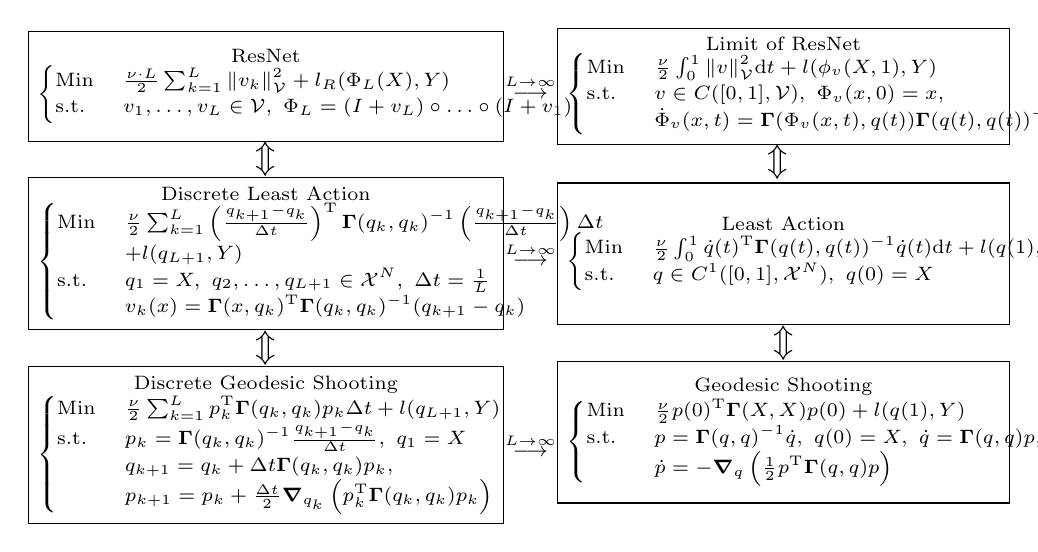
\begin{tikzpicture}[font=\scriptsize, align=center, node distance = 6mm and 6mm]
				\node[draw, above left, align=center, text width=58mm, minimum height=14mm] (a) {
					ResNet\\
					$\begin{cases}
						\text{Min~} & \frac{\nu \cdot L}{2} \sum_{k=1}^{L} \norm{v_k}_\cV^2
						+ l_R(\Phi_L(X), Y) \\
						\text{s.t.~} & v_1, \ldots, v_L \in \cV,\ \Phi_L = (I + v_L) \circ \ldots \circ (I + v_1)
					\end{cases}$};
				\node[right=of a, align=center,outer sep=-2em] (z1) {$\stackrel{L \rightarrow \infty}{\longrightarrow}$};
				\node[draw, right= of z1, align=center,text width=55mm, minimum height=14mm] (b) {
					Limit of ResNet\\
					$\begin{cases}
						\text{Min~}& \frac{\nu}{2} \int_{0}^{1} \norm{v}_\mathcal{V}^2 \mathrm{d}t
						+ l(\phi_v(X, 1), Y)\\
						\text{s.t.~}& v \in C([0, 1], \mathcal{V}),\ \Phi_v(x, 0) = x,\\
						&\dot{\Phi}_v(x, t) = \mathbf{\Gamma}(\Phi_v(x, t), q(t)) \bGamma(q(t), q(t))^{-1} \dot{q}(t)
					\end{cases}$};
				\node[below= of a,outer sep=-2em] (z2) {\large{$\Updownarrow$}};
				\node[draw, below= of z2, align=center, text width=58mm, minimum height=18mm] (c) {
					Discrete Least Action\\
					$\begin{cases}
						\text{Min~} & \frac{\nu}{2} \sum_{k=1}^{L} \left(\frac{q_{k+1} - q_k}{\Delta t}\right)^\mathrm{T} \bGamma(q_k, q_k)^{-1} \left(\frac{q_{k+1} - q_k}{\Delta t}\right) \Delta t\\
						&+ l(q_{L+1}, Y) \\
						\text{s.t.~} & q_1 = X,\ q_2, \ldots, q_{L+1} \in \cX^N,\ \Delta t = \frac{1}{L}\\
						& v_k(x) = \bGamma(x, q_k)^\mathrm{T}\bGamma(q_k, q_k)^{-1} (q_{k+1} - q_k)
					\end{cases}$};
				\node[below= of b,outer sep=-2em] (z3) {\large{$\Updownarrow$} };
				\node[right=of c, align=center,outer sep=-2em] (z4) {$\stackrel{L \rightarrow \infty}{\longrightarrow}$};
				\node[draw, below= of z3, right=of z4, align=center, text width=55mm, minimum height=18mm] (d) {
					Least Action\\
					$\begin{cases}
					\text{Min~} & \frac{\nu}{2} \int_{0}^{1} \dot{q}(t)^\mathrm{T} \mathbf{\Gamma}(q(t), q(t))^{-1}  \dot{q}(t) \mathrm{d}t + l(q(1), Y)\\
					\text{s.t.~} & q \in C^1([0,1], \cX^N),\ q(0) = X
					\end{cases}$};
				\node[below= of d,outer sep=-2em] (z5) {\large{$\Updownarrow$}};
				\node[draw, below= of z5, align=center, text width=55mm, minimum height=18mm] (e) {
					Geodesic Shooting\\
					$\begin{cases}
						\text{Min~} & \frac{\nu}{2} p(0)^\T \bGamma(X, X)p(0) + l(q(1), Y)\\
						\text{s.t.~} & 	p = \bGamma(q, q)^{-1}\dot{q},\ q(0) = X,\ \dot{q} = \bGamma(q, q) p,\\
						&\dot{p} = -\grad_q \left(\frac{1}{2} p^\mathrm{T} \bGamma(q, q) p\right)
					\end{cases}$};
				\node[below= of c,outer sep=-2em] (z6) {\large{$\Updownarrow$}};
				\node[draw, below= of z6, align=center, text width=58mm, minimum height=18mm] (f) {
					Discrete Geodesic Shooting\\
					$\begin{cases}
					\text{Min~} & \frac{\nu}{2} \sum_{k=1}^L p_k^\T \bGamma(q_k, q_k) p_k \Delta t + l(q_{L+1}, Y)\\
					\text{s.t.~} & p_k = \bGamma(q_k, q_k)^{-1} \frac{q_{k+1} - q_k}{\Delta t},\ q_1 = X \\
					& q_{k+1} = q_k + \Delta t \bGamma(q_k, q_k) p_k,\\
					& p_{k+1} = p_k + \frac{\Delta t}{2} \grad_{q_k} \left(p_k^\T \bGamma(q_k, q_k) p_k\right)
					\end{cases}$};
				\node[right=of f, align=center,outer sep=-2em] (z7) {$\stackrel{L \rightarrow \infty}{\longrightarrow}$};
		\end{tikzpicture}
	}
	\label{fig:convergence}
\end{figure}
	\end{frame}

	\begin{frame}{Algorithm}
		Choose a loss function $l$, kernels $\Gamma$ and $K$ and a balancing parameter $\nu$.\\
		Choose an initial momentum $p_0$.
		
		Modified Leapfrog scheme:
		\begin{align*}
			p_{n+\frac{1}{2}} &\gets p_n - \frac{h}{2} \grad_q\fH\left(q_n, p_n\right) \\
			q_{n+1} &\gets q_n + h \grad_p\fH\left(q_n, p_{n+\frac{1}{2}}\right)\\
			p_{n+1} &\gets p_{n+\frac{1}{2}} - \frac{h}{2} \grad_q\fH\left(q_{n+1}, p_{n+\frac{1}{2}}\right) \ .
		\end{align*}
		
		Use $q(1)$ and $p(0)$ to compute and minimize
		\begin{equation*}
			\frac{\nu}{2} p(0)^\T \mathbf{\Gamma}(X, X)p(0) + l(q(1), Y) \ .
		\end{equation*}
		via gradient descent.
%		\begin{enumerate}[label=\arabic*.]
%			\item Choose a loss function $l$, kernels $\Gamma$ and $K$ and a balancing parameter $\nu$.
%			\item Choose an initial momentum $p_0$.
%			\item Minimize $\frac{\nu}{2} p(0)^\T \mathbf{\Gamma}(X, X)p(0) + l(q(1), Y)$ by iterating the following steps:
%			\begin{enumerate}[label=3.\arabic*.]
%				\item Solve the Hamiltonian system  with initial conditions $q(0) = X$, $p(0) = p_0$.
%				\item Compute $q(1)$ and with that, the gradient of $\frac{\nu}{2} p(0)^\T \mathbf{\Gamma}(X, X)p(0) + l(q(1), Y)$ with respect to $p(0)$.
%				\item Update $p(0)$ through gradient descent.
%			\end{enumerate}
%			\item Solve the differential equation with $q(0) = X$ and the optimal momentum $p(0)$ computed above to obtain $\Phi_v(\cdot, 1): \cX \rightarrow \cX$.
%			\item Compute $f: \cX \rightarrow \cY$ as the minimizer of $l(\Phi_v(X, 1), Y)$ and approximate the target function $f^\dagger$ with $f \circ \Phi_v(\cdot, 1)$.
%		\end{enumerate}
	\end{frame}

	\begin{frame}{Swiss Roll Dataset}
		\begin{figure}
	\caption{The Swiss Roll dataset.}
	\label{fig:dataset}
\end{figure}
	\end{frame}

	\begin{frame}{Experimental Results}
		\begin{figure}
	\makebox[\textwidth][c]{
		\centering
		\def\imagescale{0.15}
		\begin{tikzpicture}[node distance=-0.25cm and -0.45cm, font=\scriptsize]
			\node [] (b1) {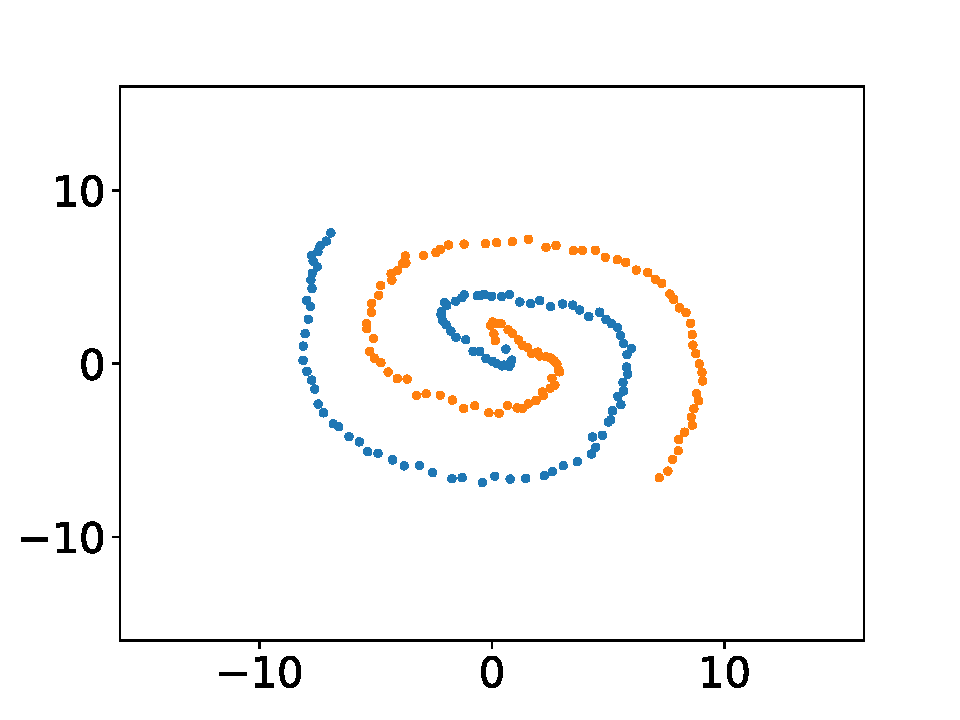
\includegraphics[scale=\imagescale]{presentation/results/best_ckpt_2021_01_14_s_5_r_0.1_h_0.2_mu_0.01_reg_1e-06_step_0.2.pdf}}; 
			\node [right= of b1] (b2) {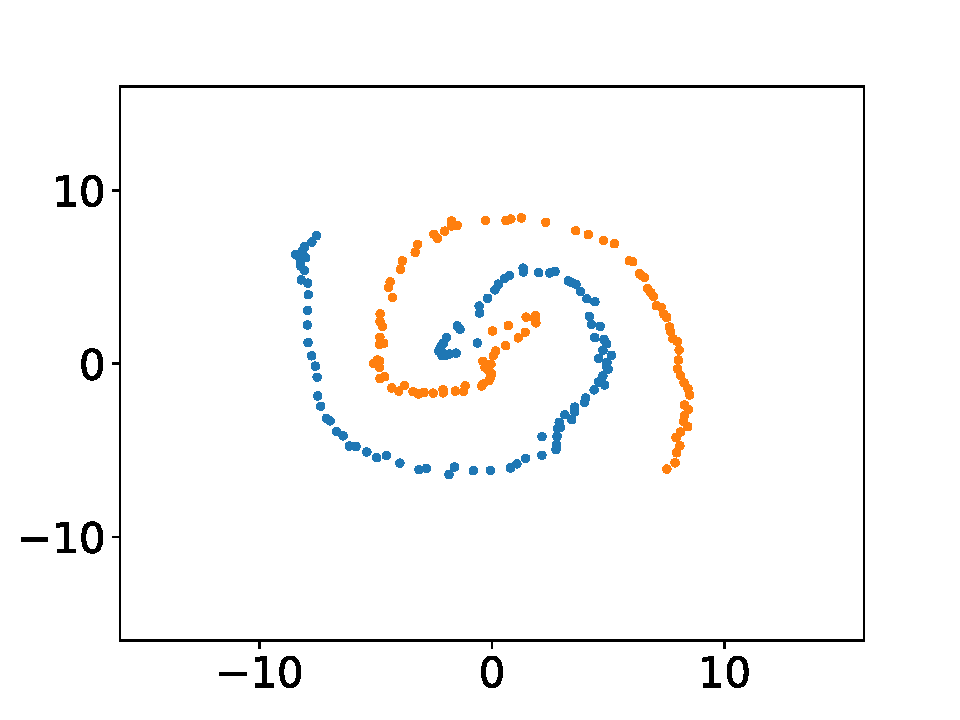
\includegraphics[scale=\imagescale]{presentation/results/best_ckpt_2021_01_14_s_5_r_0.1_h_0.2_mu_0.01_reg_1e-06_step_0.4.pdf}};
			\node [right= of b2] (b3) {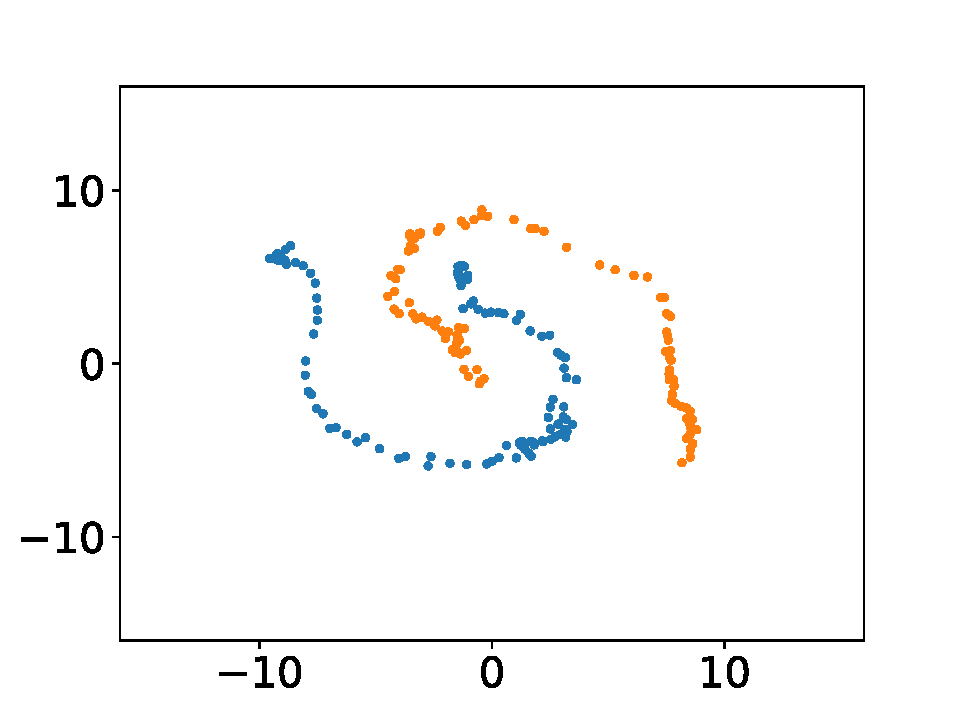
\includegraphics[scale=\imagescale]{presentation/results/best_ckpt_2021_01_14_s_5_r_0.1_h_0.2_mu_0.01_reg_1e-06_step_0.6.pdf}};
			\node [right= of b3] (b4) {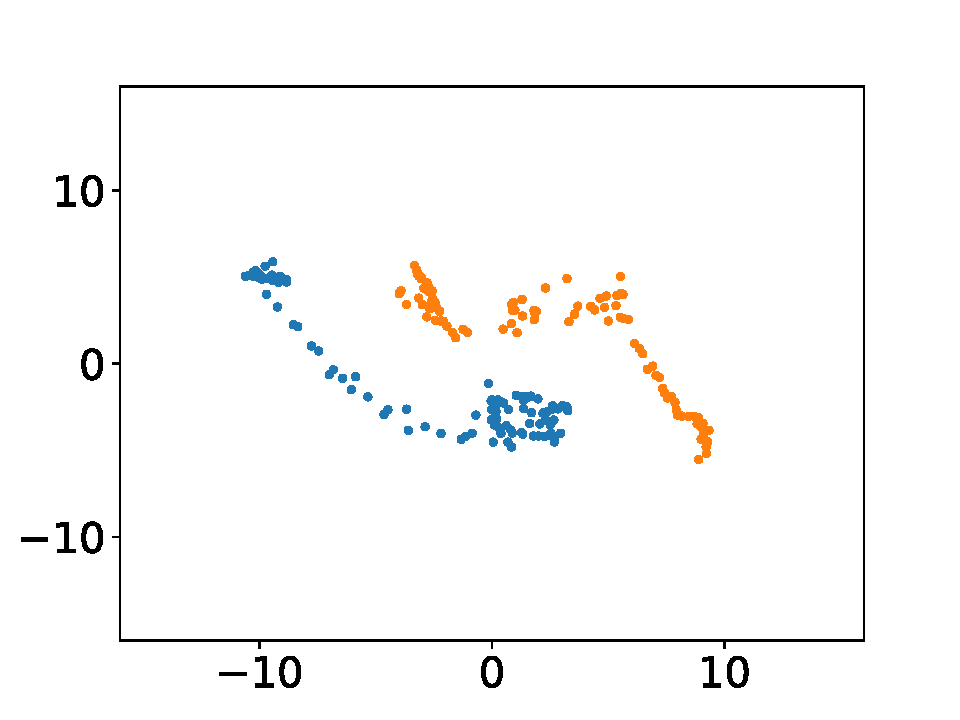
\includegraphics[scale=\imagescale]{presentation/results/best_ckpt_2021_01_14_s_5_r_0.1_h_0.2_mu_0.01_reg_1e-06_step_0.8.pdf}};
			\node [right= of b4] (b5) {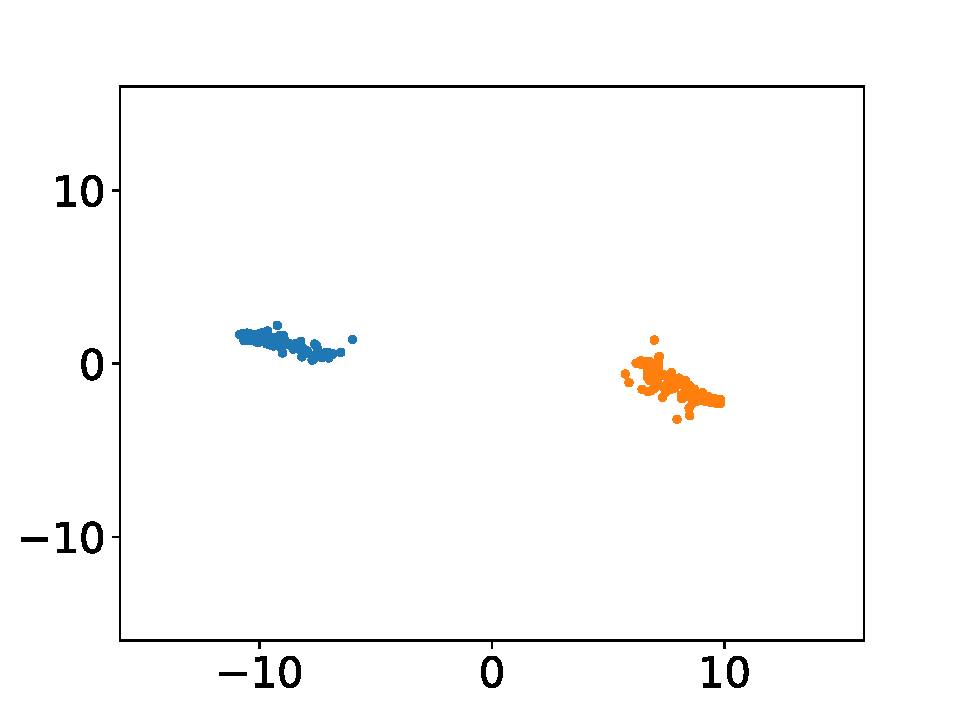
\includegraphics[scale=\imagescale]{presentation/results/best_ckpt_2021_01_14_s_5_r_0.1_h_0.2_mu_0.01_reg_1e-06_step_1.0.pdf}};
			%
			\node [below= of b1] (c1) {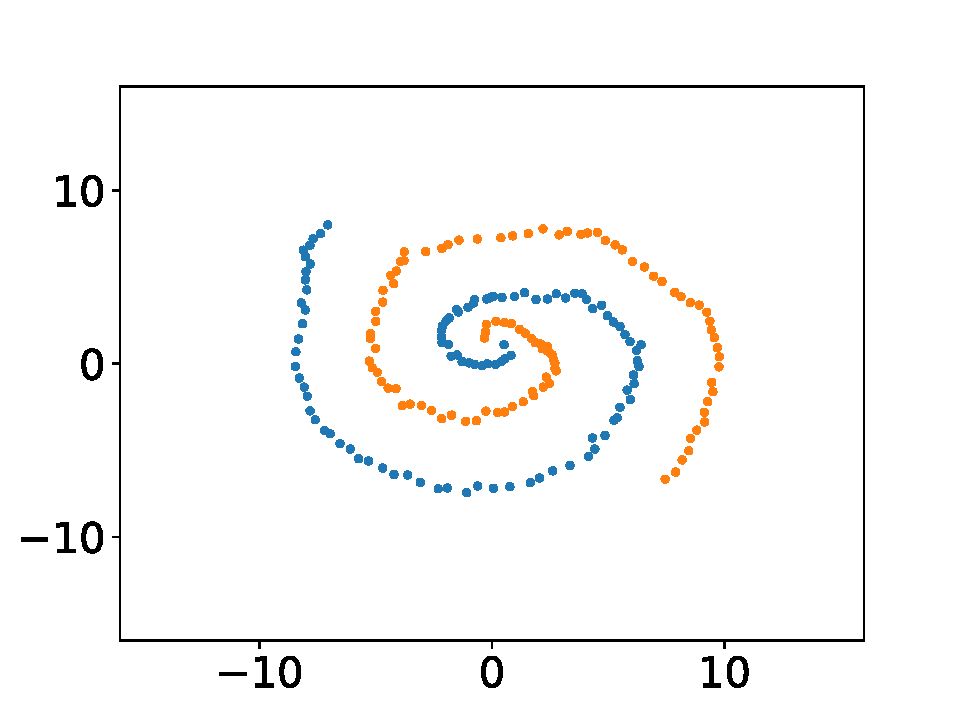
\includegraphics[scale=\imagescale]{presentation/results/best_ckpt_2021_01_14_s_5_r_0.1_h_0.2_mu_0.02_reg_1e-06_step_0.2.pdf}}; 
			\node [right= of c1] (c2) {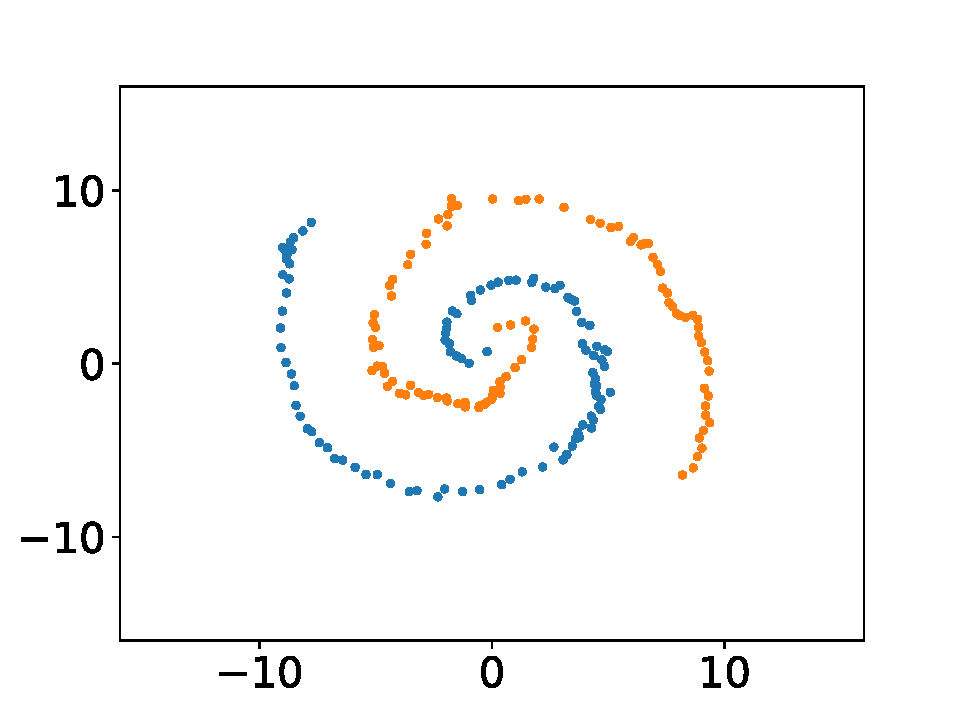
\includegraphics[scale=\imagescale]{presentation/results/best_ckpt_2021_01_14_s_5_r_0.1_h_0.2_mu_0.02_reg_1e-06_step_0.4.pdf}};
			\node [right= of c2] (c3) {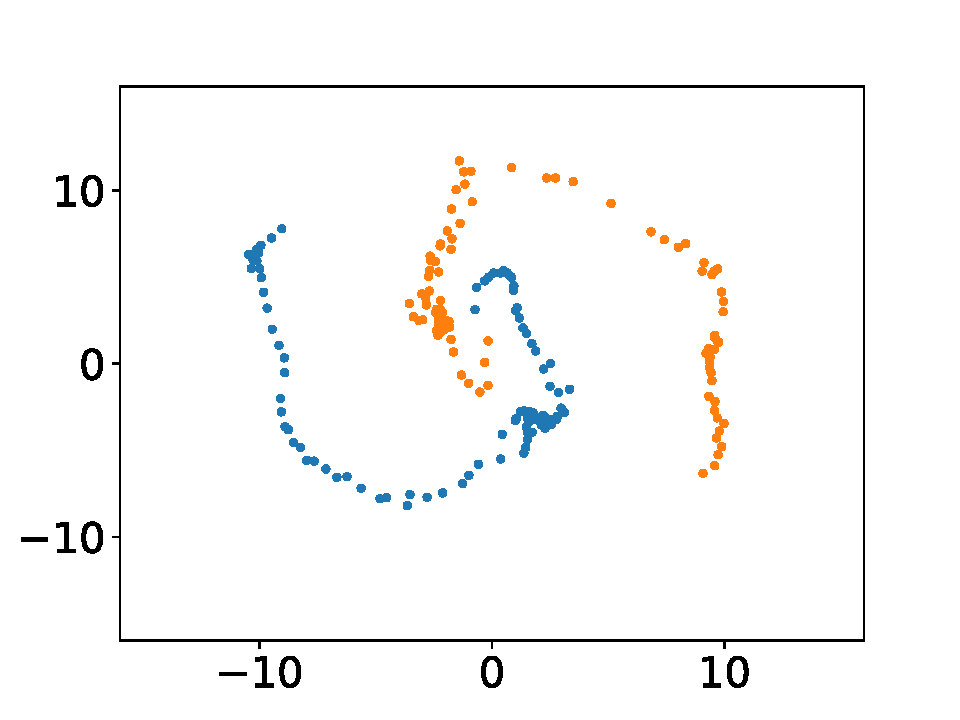
\includegraphics[scale=\imagescale]{presentation/results/best_ckpt_2021_01_14_s_5_r_0.1_h_0.2_mu_0.02_reg_1e-06_step_0.6.pdf}};
			\node [right= of c3] (c4) {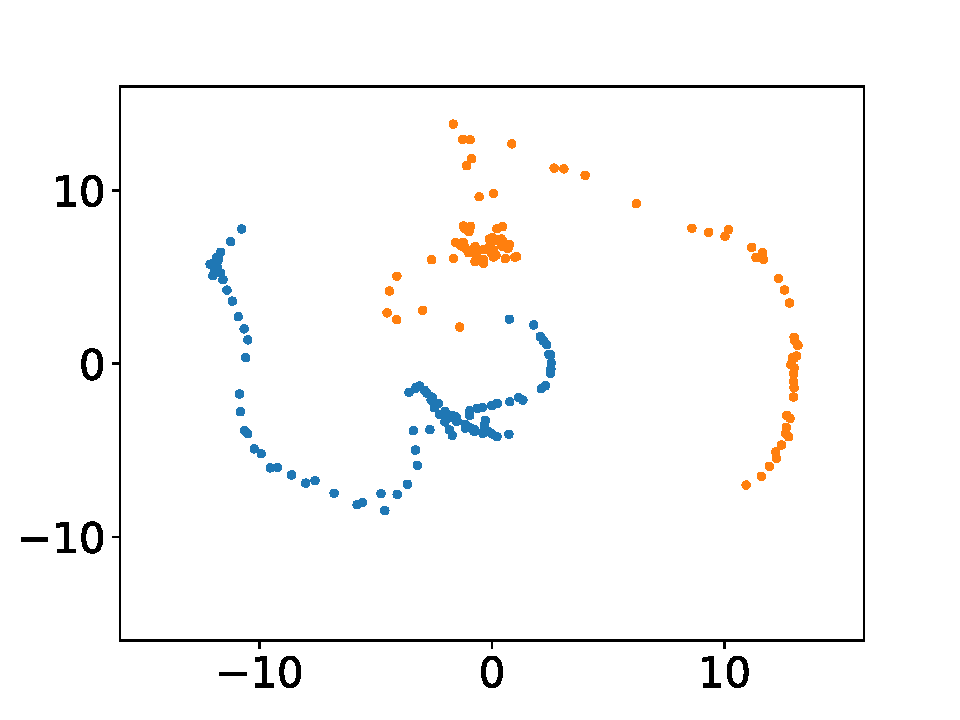
\includegraphics[scale=\imagescale]{presentation/results/best_ckpt_2021_01_14_s_5_r_0.1_h_0.2_mu_0.02_reg_1e-06_step_0.8.pdf}};
			\node [right= of c4] (c5) {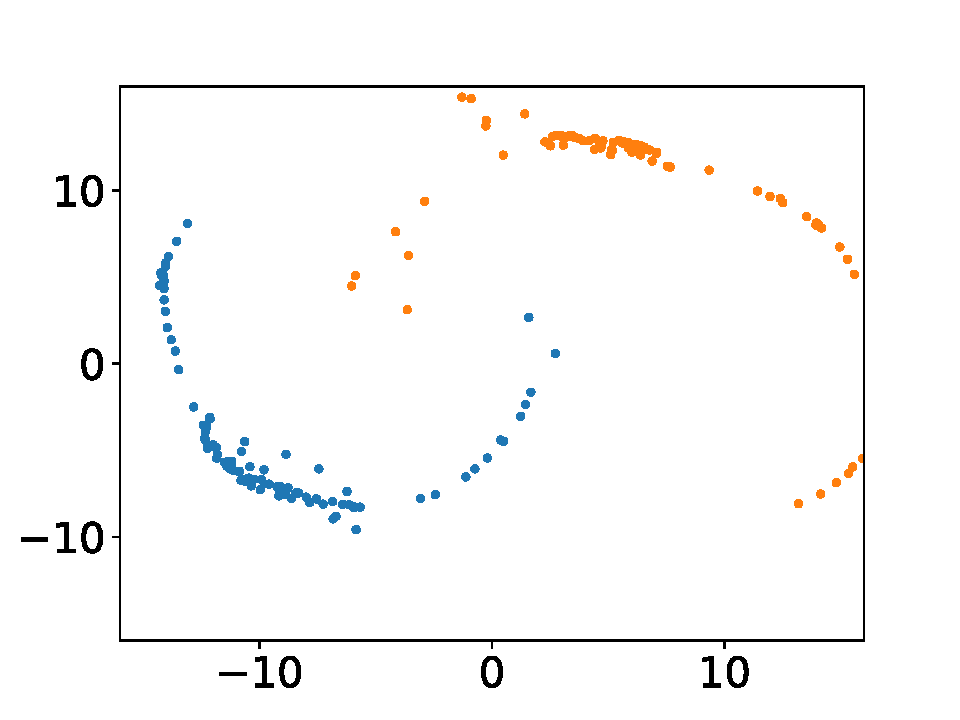
\includegraphics[scale=\imagescale]{presentation/results/best_ckpt_2021_01_14_s_5_r_0.1_h_0.2_mu_0.02_reg_1e-06_step_1.0.pdf}};
			%
			\node [below= of c1] (d1) {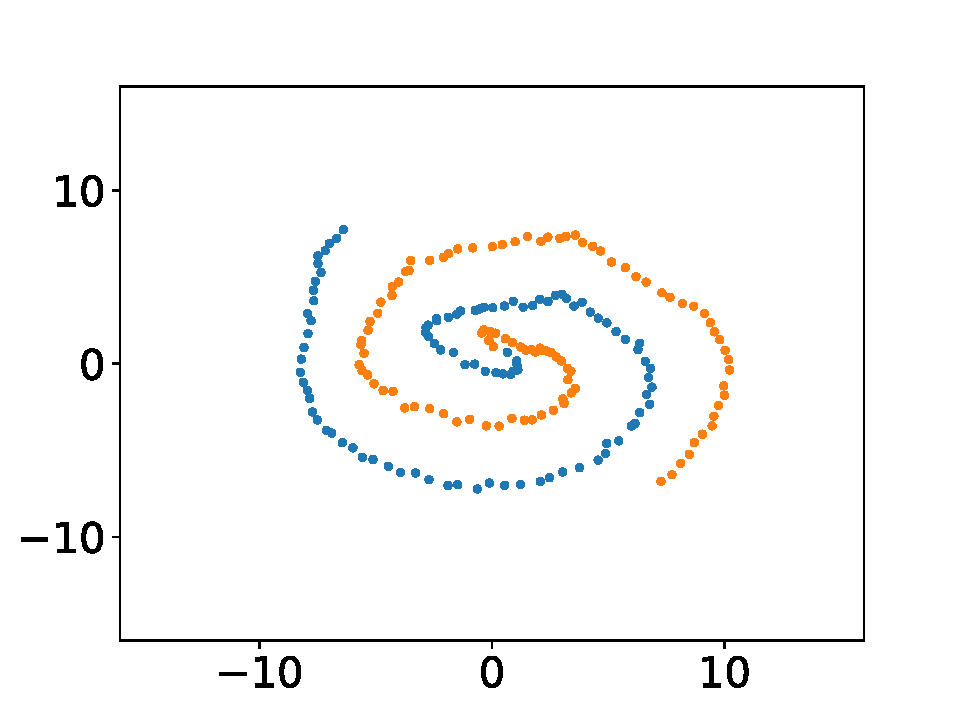
\includegraphics[scale=\imagescale]{presentation/results/best_ckpt_2021_01_14_s_5_r_0.1_h_0.2_mu_0.03_reg_1e-06_step_0.2.pdf}}; 
			\node [right= of d1] (d2) {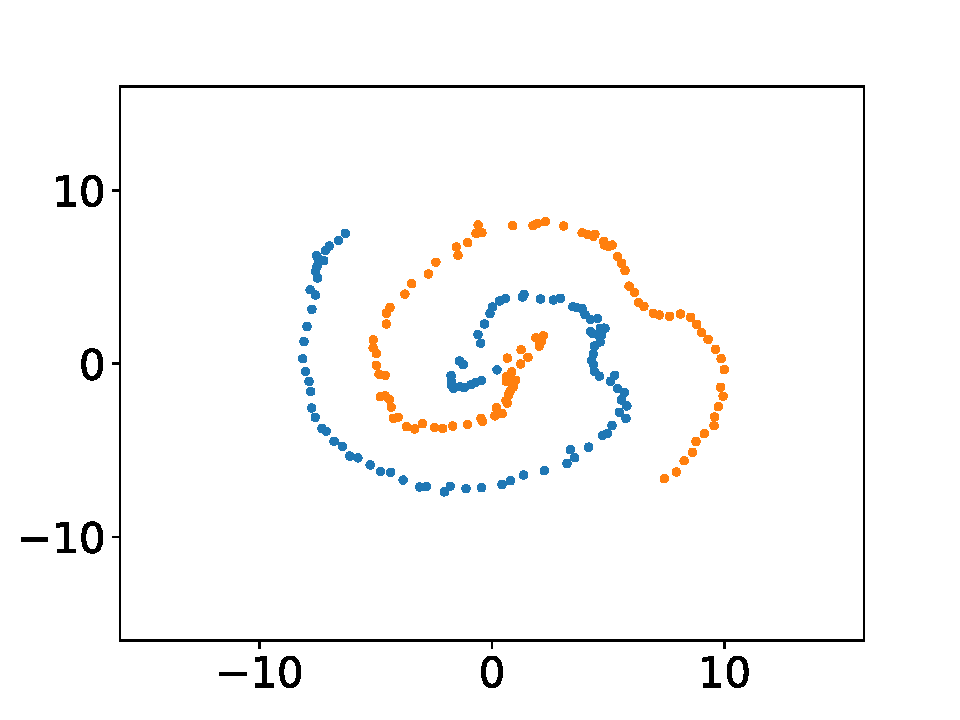
\includegraphics[scale=\imagescale]{presentation/results/best_ckpt_2021_01_14_s_5_r_0.1_h_0.2_mu_0.03_reg_1e-06_step_0.4.pdf}};
			\node [right= of d2] (d3) {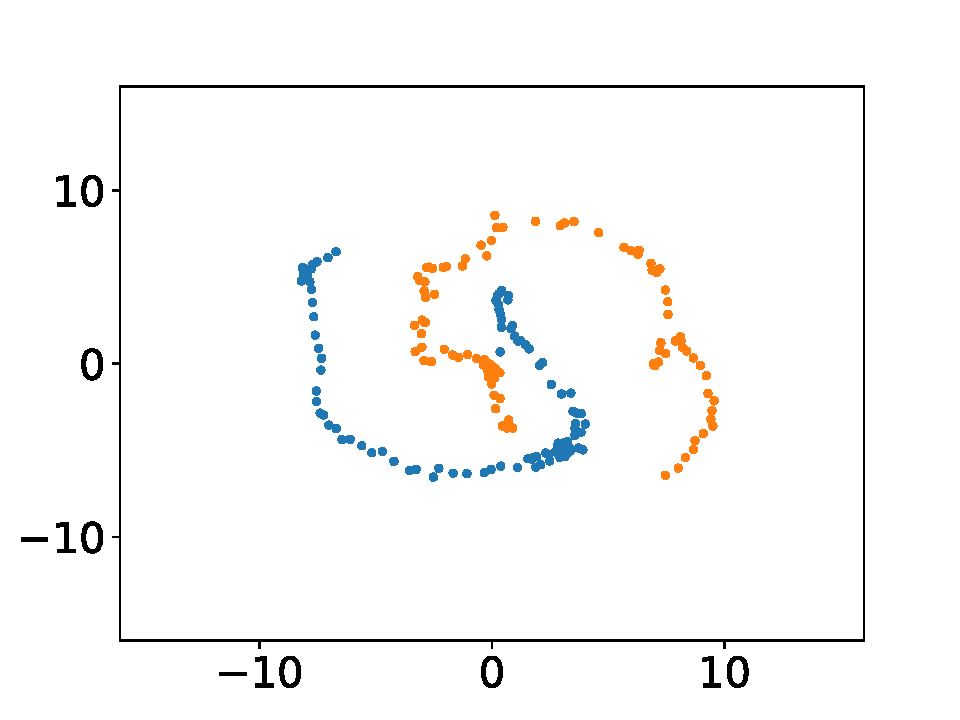
\includegraphics[scale=\imagescale]{presentation/results/best_ckpt_2021_01_14_s_5_r_0.1_h_0.2_mu_0.03_reg_1e-06_step_0.6.pdf}};
			\node [right= of d3] (d4) {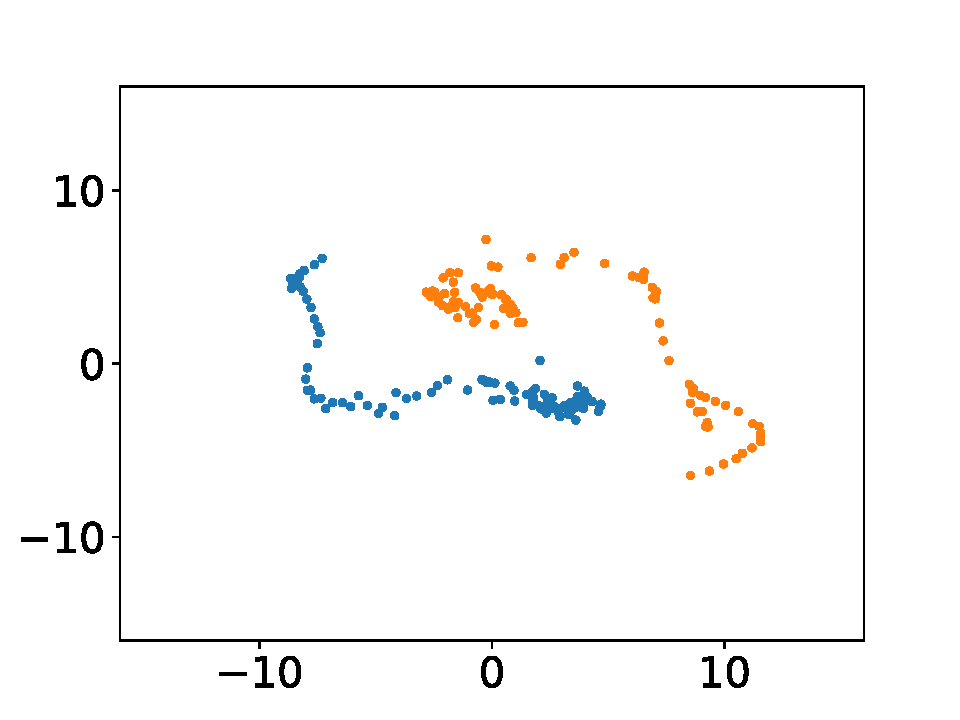
\includegraphics[scale=\imagescale]{presentation/results/best_ckpt_2021_01_14_s_5_r_0.1_h_0.2_mu_0.03_reg_1e-06_step_0.8.pdf}};
			\node [right= of d4] (d5) {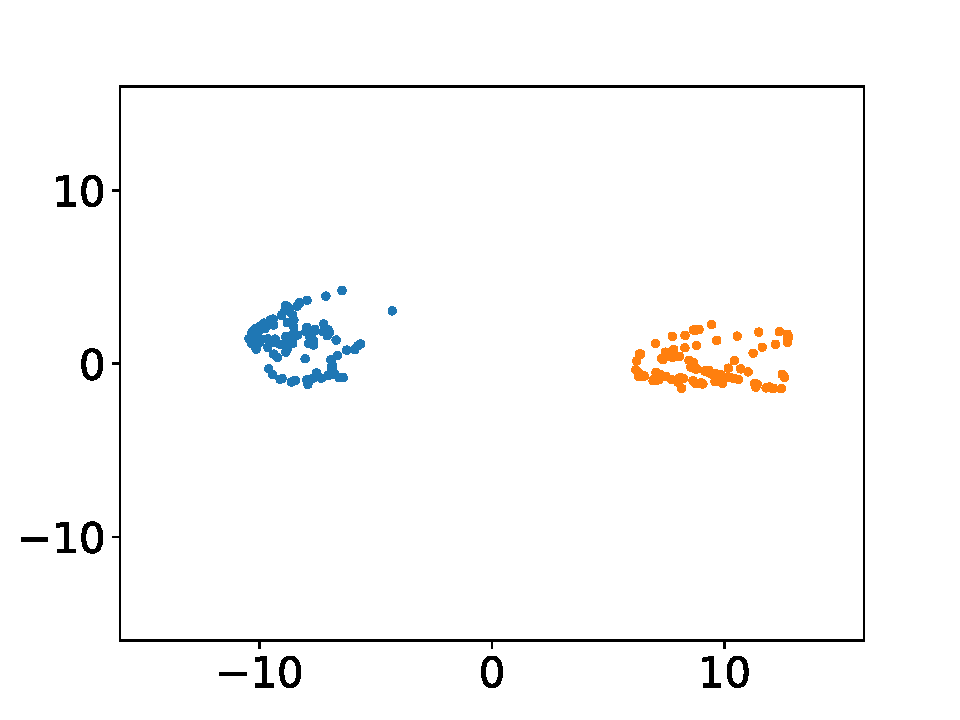
\includegraphics[scale=\imagescale]{presentation/results/best_ckpt_2021_01_14_s_5_r_0.1_h_0.2_mu_0.03_reg_1e-06_step_1.0.pdf}};
			%
			\node [below= of d1] (e1) {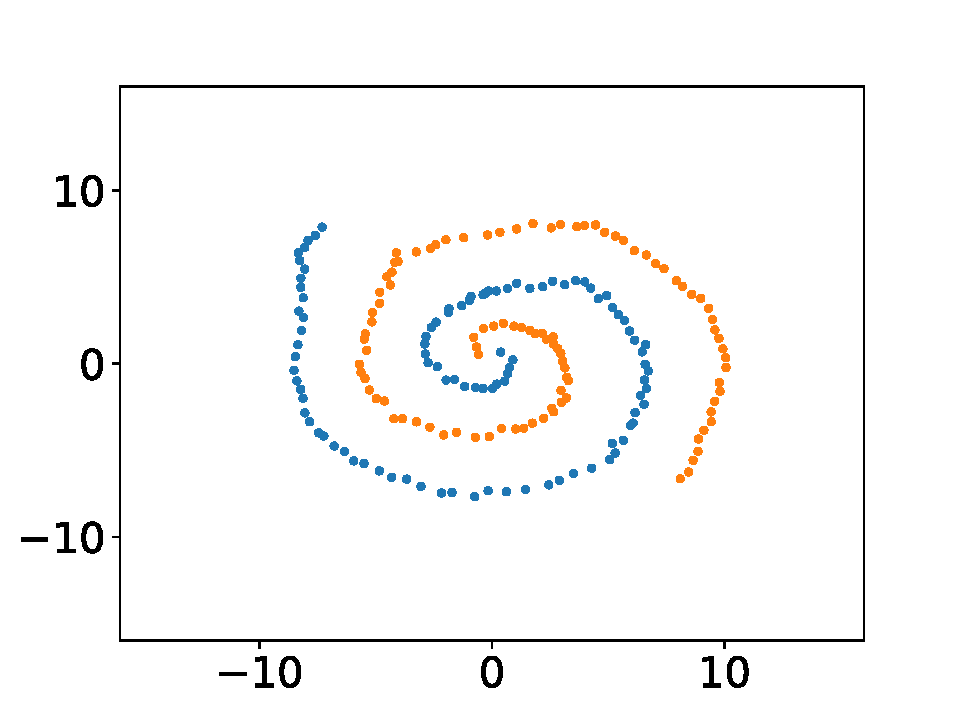
\includegraphics[scale=\imagescale]{presentation/results/best_ckpt_2021_01_14_s_5_r_0.1_h_0.2_mu_0.05_reg_1e-06_step_0.2.pdf}}; 
			\node [right= of e1] (e2) {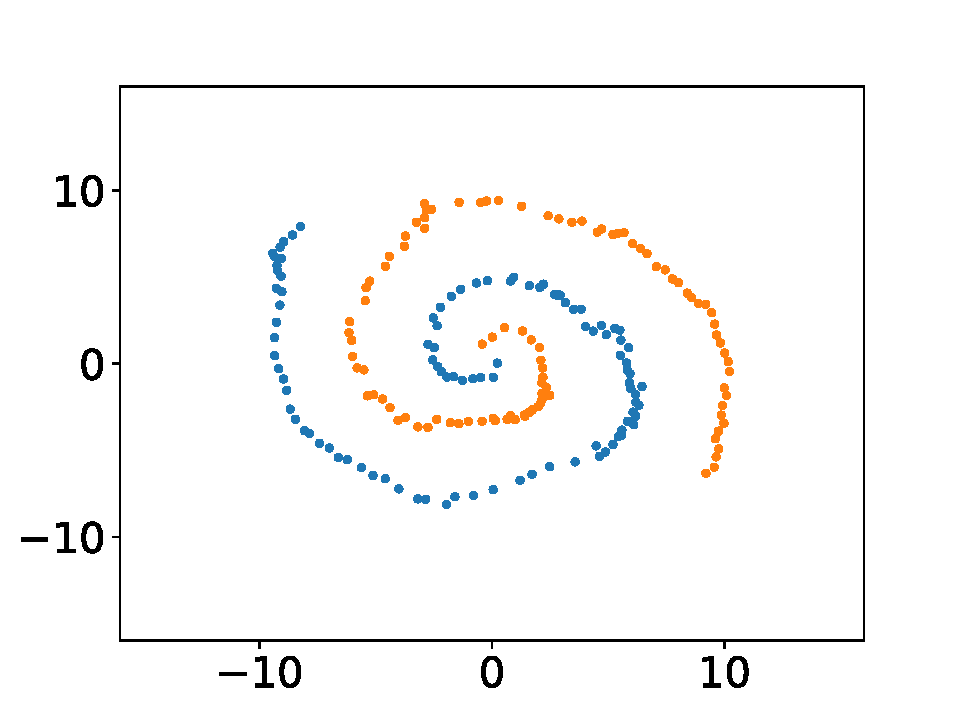
\includegraphics[scale=\imagescale]{presentation/results/best_ckpt_2021_01_14_s_5_r_0.1_h_0.2_mu_0.05_reg_1e-06_step_0.4.pdf}};
			\node [right= of e2] (e3) {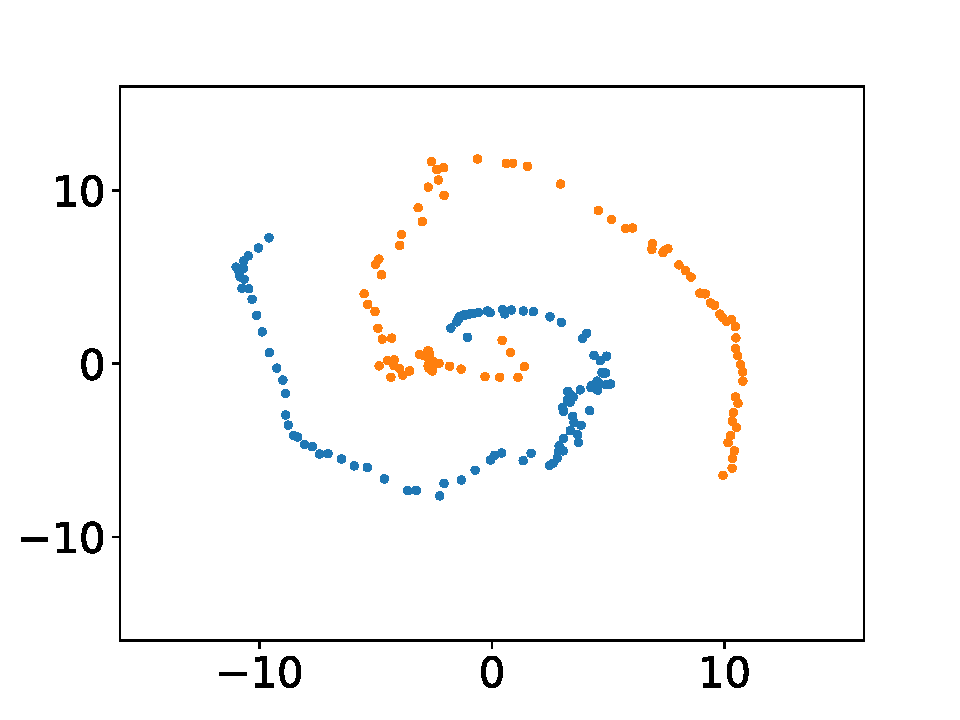
\includegraphics[scale=\imagescale]{presentation/results/best_ckpt_2021_01_14_s_5_r_0.1_h_0.2_mu_0.05_reg_1e-06_step_0.6.pdf}};
			\node [right= of e3] (e4) {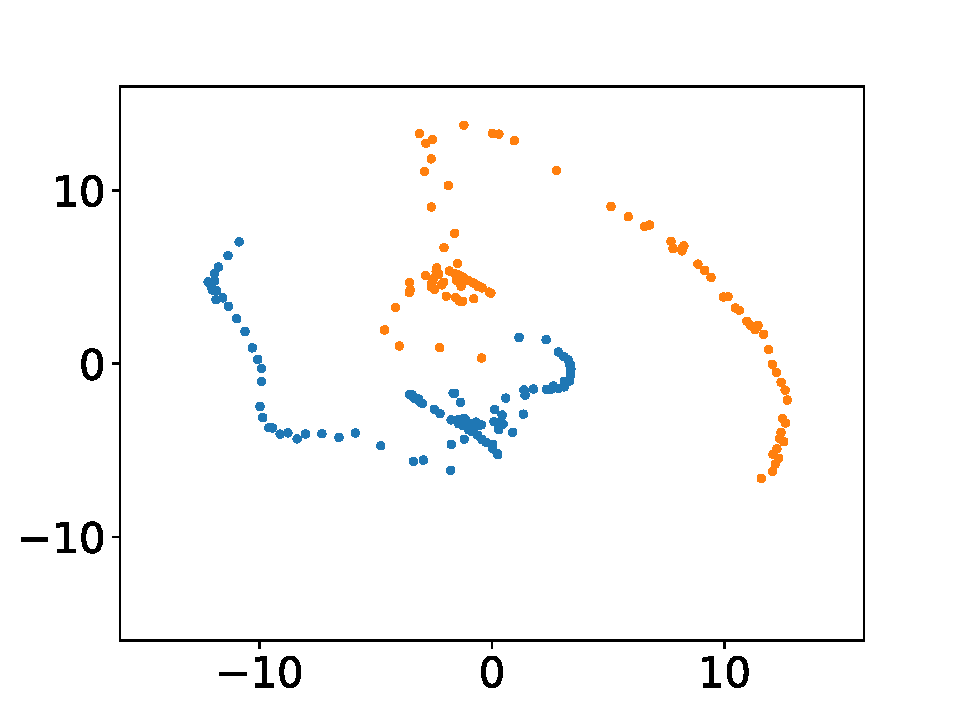
\includegraphics[scale=\imagescale]{presentation/results/best_ckpt_2021_01_14_s_5_r_0.1_h_0.2_mu_0.05_reg_1e-06_step_0.8.pdf}};
			\node [right= of e4] (e5) {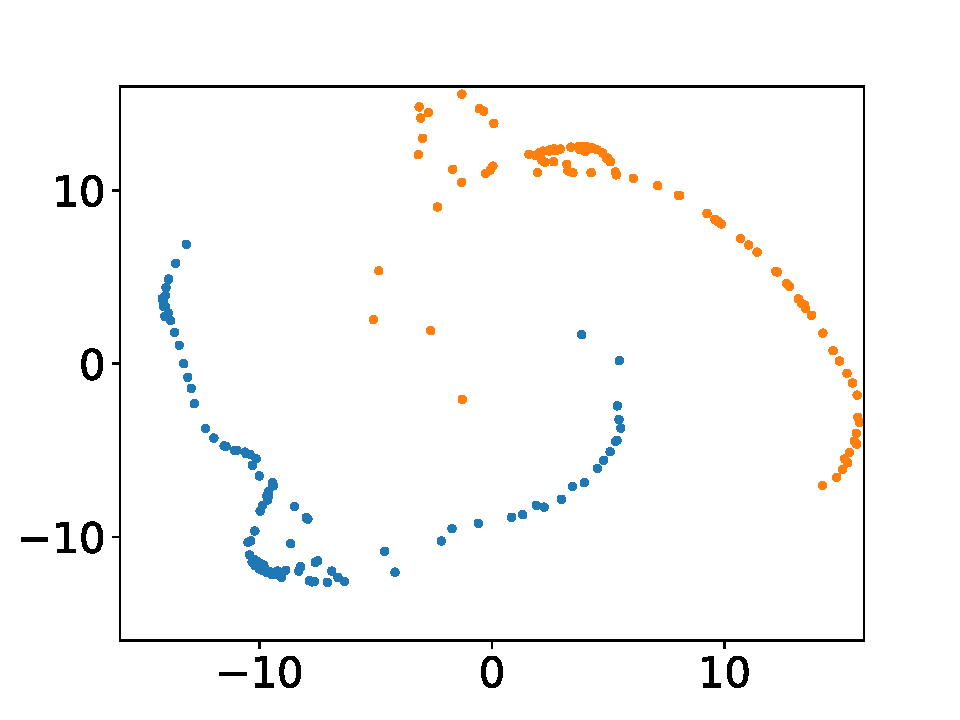
\includegraphics[scale=\imagescale]{presentation/results/best_ckpt_2021_01_14_s_5_r_0.1_h_0.2_mu_0.05_reg_1e-06_step_1.0.pdf}};
			%
			\node[left= -0.1cm of b1] (b0) {$\nu=0.01$};
			\node[left= -0.1cm of c1] (c0) {$\nu=0.02$};
			\node[left= -0.1cm of d1] (d0) {$\nu=0.03$};
			\node[left= -0.1cm of e1] (e0) {$\nu=0.05$};
			%
			\node[above= -0.1cm of b1] (z1) {$t=0.2$};
			\node[above= -0.1cm of b2] (z2) {$t=0.4$};
			\node[above= -0.1cm of b3] (z3) {$t=0.6$};
			\node[above= -0.1cm of b4] (z4) {$t=0.8$};
			\node[above= -0.1cm of b5] (z5) {$t=1$};
		\end{tikzpicture}
	}
\end{figure}
	\end{frame}


	\begin{frame}
		\bibliography{bibliography}
		\bibliographystyle{plainnat}
	\end{frame}
\end{document}